%author:  Wentai ZHANG(rchardx@gmail.com)

\input{ctex4xetex.cfg}
\documentclass{ctexrep}

\usepackage[CJKtextspaces]{xeCJK}
% Copyright(C) 2008,2009 Wentai ZHANG
% Default OpenType Font Configuration for xeCJK

\defaultfontfeatures{Mapping=tex-text}

\def\cjkrm{Adobe Song Std}
\def\cjksf{Adobe Kaiti Std}
\def\cjktt{Adobe Fangsong Std}

\def\cjkbd{Adobe Heiti Std}
\def\cjkit{Adobe Kaiti Std}

\setCJKfamilyfont{rm}[BoldFont=\cjkbd,ItalicFont=\cjkit]{\cjkrm}
\setCJKfamilyfont{sf}[BoldFont=\cjkbd,ItalicFont=\cjkit]{\cjksf}
\setCJKfamilyfont{tt}[BoldFont=\cjkbd,ItalicFont=\cjkit]{\cjktt}

\setCJKmainfont[BoldFont=\cjkbd,ItalicFont=\cjkit]{\cjkrm}
\setCJKsansfont[BoldFont=\cjkbd,ItalicFont=\cjkit]{\cjksf}
\setCJKmonofont[BoldFont=\cjkbd,ItalicFont=\cjkit]{\cjktt}

\setmainfont{TeX Gyre Pagella}
\setsansfont{TeX Gyre Adventor}
\setmonofont{TeX Gyre Cursor}
% \setmainfont{Arno Pro}
% \setsansfont{Myriad Pro}
% \setmonofont{Courier Std}


\usepackage{amsmath,amssymb,amsthm,latexsym,mathrsfs}
\usepackage{graphicx}

\newcommand{\bbold}[1]{\textbf{#1}}

\begin{document}
\title{JSOI2010冬令营数论练习赛}
\author{张文泰}
\maketitle

\newpage
\section*{Farey数列farey}

\subsection*{问题描述}
我们令Farey数列$F_n$表示所有分母不大于$n$的既约真分数集合。
比如$F_5=\{1/5,1/4,1/3,2/5,1/2,3/5,2/3,3/4,4/5\}$。
现在给定$n$和$k$,求出$F_n$中的第$k$大的项。

\paragraph{限制} 时间:2000MS;内存:64MB

\paragraph{输入格式}
输入文件中仅一行为两个数$n$和$k$,保证合法。

\paragraph{输出格式}
输出文件中仅一行为两个数$P$和$Q$,表示第$k$项是$P/Q$。

\subsection*{输入样例farey.in}
\begin{verbatim}
5 6
\end{verbatim}

\subsection*{输出样例farey.out}
\begin{verbatim}
3 5
\end{verbatim}

\subsection*{数据范围}
$1<n\leq 40000$;
对于$40\%$的数据,$k\leq 50000$;
对于$100\%$的数据,$n\geq 10000$。

\newpage
\section*{公约数求和sum}

\subsection*{问题描述}
给定一个$N(1<N<2^{31})$,求$\displaystyle\sum_{i=1}^N (i,N)$。

\paragraph{限制} 时间:1000MS;内存:64MB

\paragraph{输入格式}
输入数据有多个,一行一个正整数表示$N$。输入数据不会超过10000个。

\paragraph{输出格式}
输出所有的和,一行一个。

\subsection*{输入样例sum.in}
\begin{verbatim}
2
6
\end{verbatim}

\subsection*{输出样例sum.out}
\begin{verbatim}
3
15
\end{verbatim}

\newpage
\section*{阶乘fact}

\subsection*{问题描述}
给定$n$,求出$n!$的最后一位非零位。

\paragraph{限制} 时间:2000MS;内存:64MB

\paragraph{输入格式}
输入数据有多个,每行一个整数表示$n(0<n<2^{31})$。数据不会超过100000组。

\paragraph{输出格式}
对于每个数据,输出相应的答案。

\subsection*{输入样例fact.in}
\begin{verbatim}
1
2
3
4
5
\end{verbatim}

\subsection*{输出样例fact.out}
\begin{verbatim}
1
2
6
4
2
\end{verbatim}

\newpage
\section*{楼梯涂色color}

\subsection*{问题描述}
我们要建造一些$N(\leq N\leq 10^9)$层的楼梯。众所周知,楼梯从上往下依次有$1,2,3,\dotsc,N$个块组成。也就是说,一个$N$层的楼梯一共有$\frac{N(N+1)}{2}$块。现在我们有许多各种各样的整块可以用来建造楼梯,我们规定,一个$N$层的楼梯只能用$N$个整块来搭建。我们举一个例子,$3$层的楼梯有$5$种方法建造:

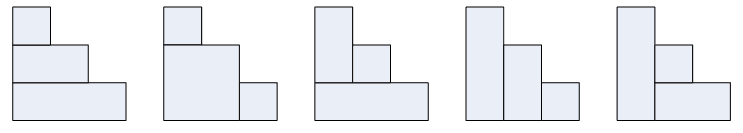
\includegraphics[scale=0.4]{staircolor.png}

现在我们有$K(\leq K\leq 10^9)$种染料,要对这所有的楼梯进行涂色。每种方案可以任意选择一种染料来涂色,所有的颜色不一定全要用上。你需要计算出涂色的总方案数,由于答案可能很大,所以请只要输出答案模$1000000123$的余数即可。

\paragraph{限制} 时间:1000MS;内存:64MB

\paragraph{输入格式}
输入会包含多组数据。每组数据仅一行,为$N,K$,程序应当处理到文件结束。每个输入数据里不会超过5个数据。

\paragraph{输出格式}
对于每组数据,输出相应的答案。

\subsection*{输入样例color.in}
\begin{verbatim}
3 2
2 2
1 1
\end{verbatim}

\subsection*{输出样例color.out}
\begin{verbatim}
32
4
1
\end{verbatim}

\subsection*{样例解释}
对于$N=3,K=2$这组数据,一共有$5$种建造方案,那么答案就是$2^5=32$。

\end{document}
